\documentclass[border=10pt]{standalone} 
\usepackage{tikz}

\usetikzlibrary{calc}
\usetikzlibrary{arrows}
\usetikzlibrary{shadows}
\usetikzlibrary{patterns}
\usetikzlibrary{positioning}
\usetikzlibrary{shapes}
\usetikzlibrary{3d}
%\usetikzlibrary{automata}
\usetikzlibrary{fit}

\tikzset{block/.style={draw, text centered, fill=gray!10,drop shadow}}
\tikzset{connect/.style={draw, line width=1 pt}}

\begin{document}


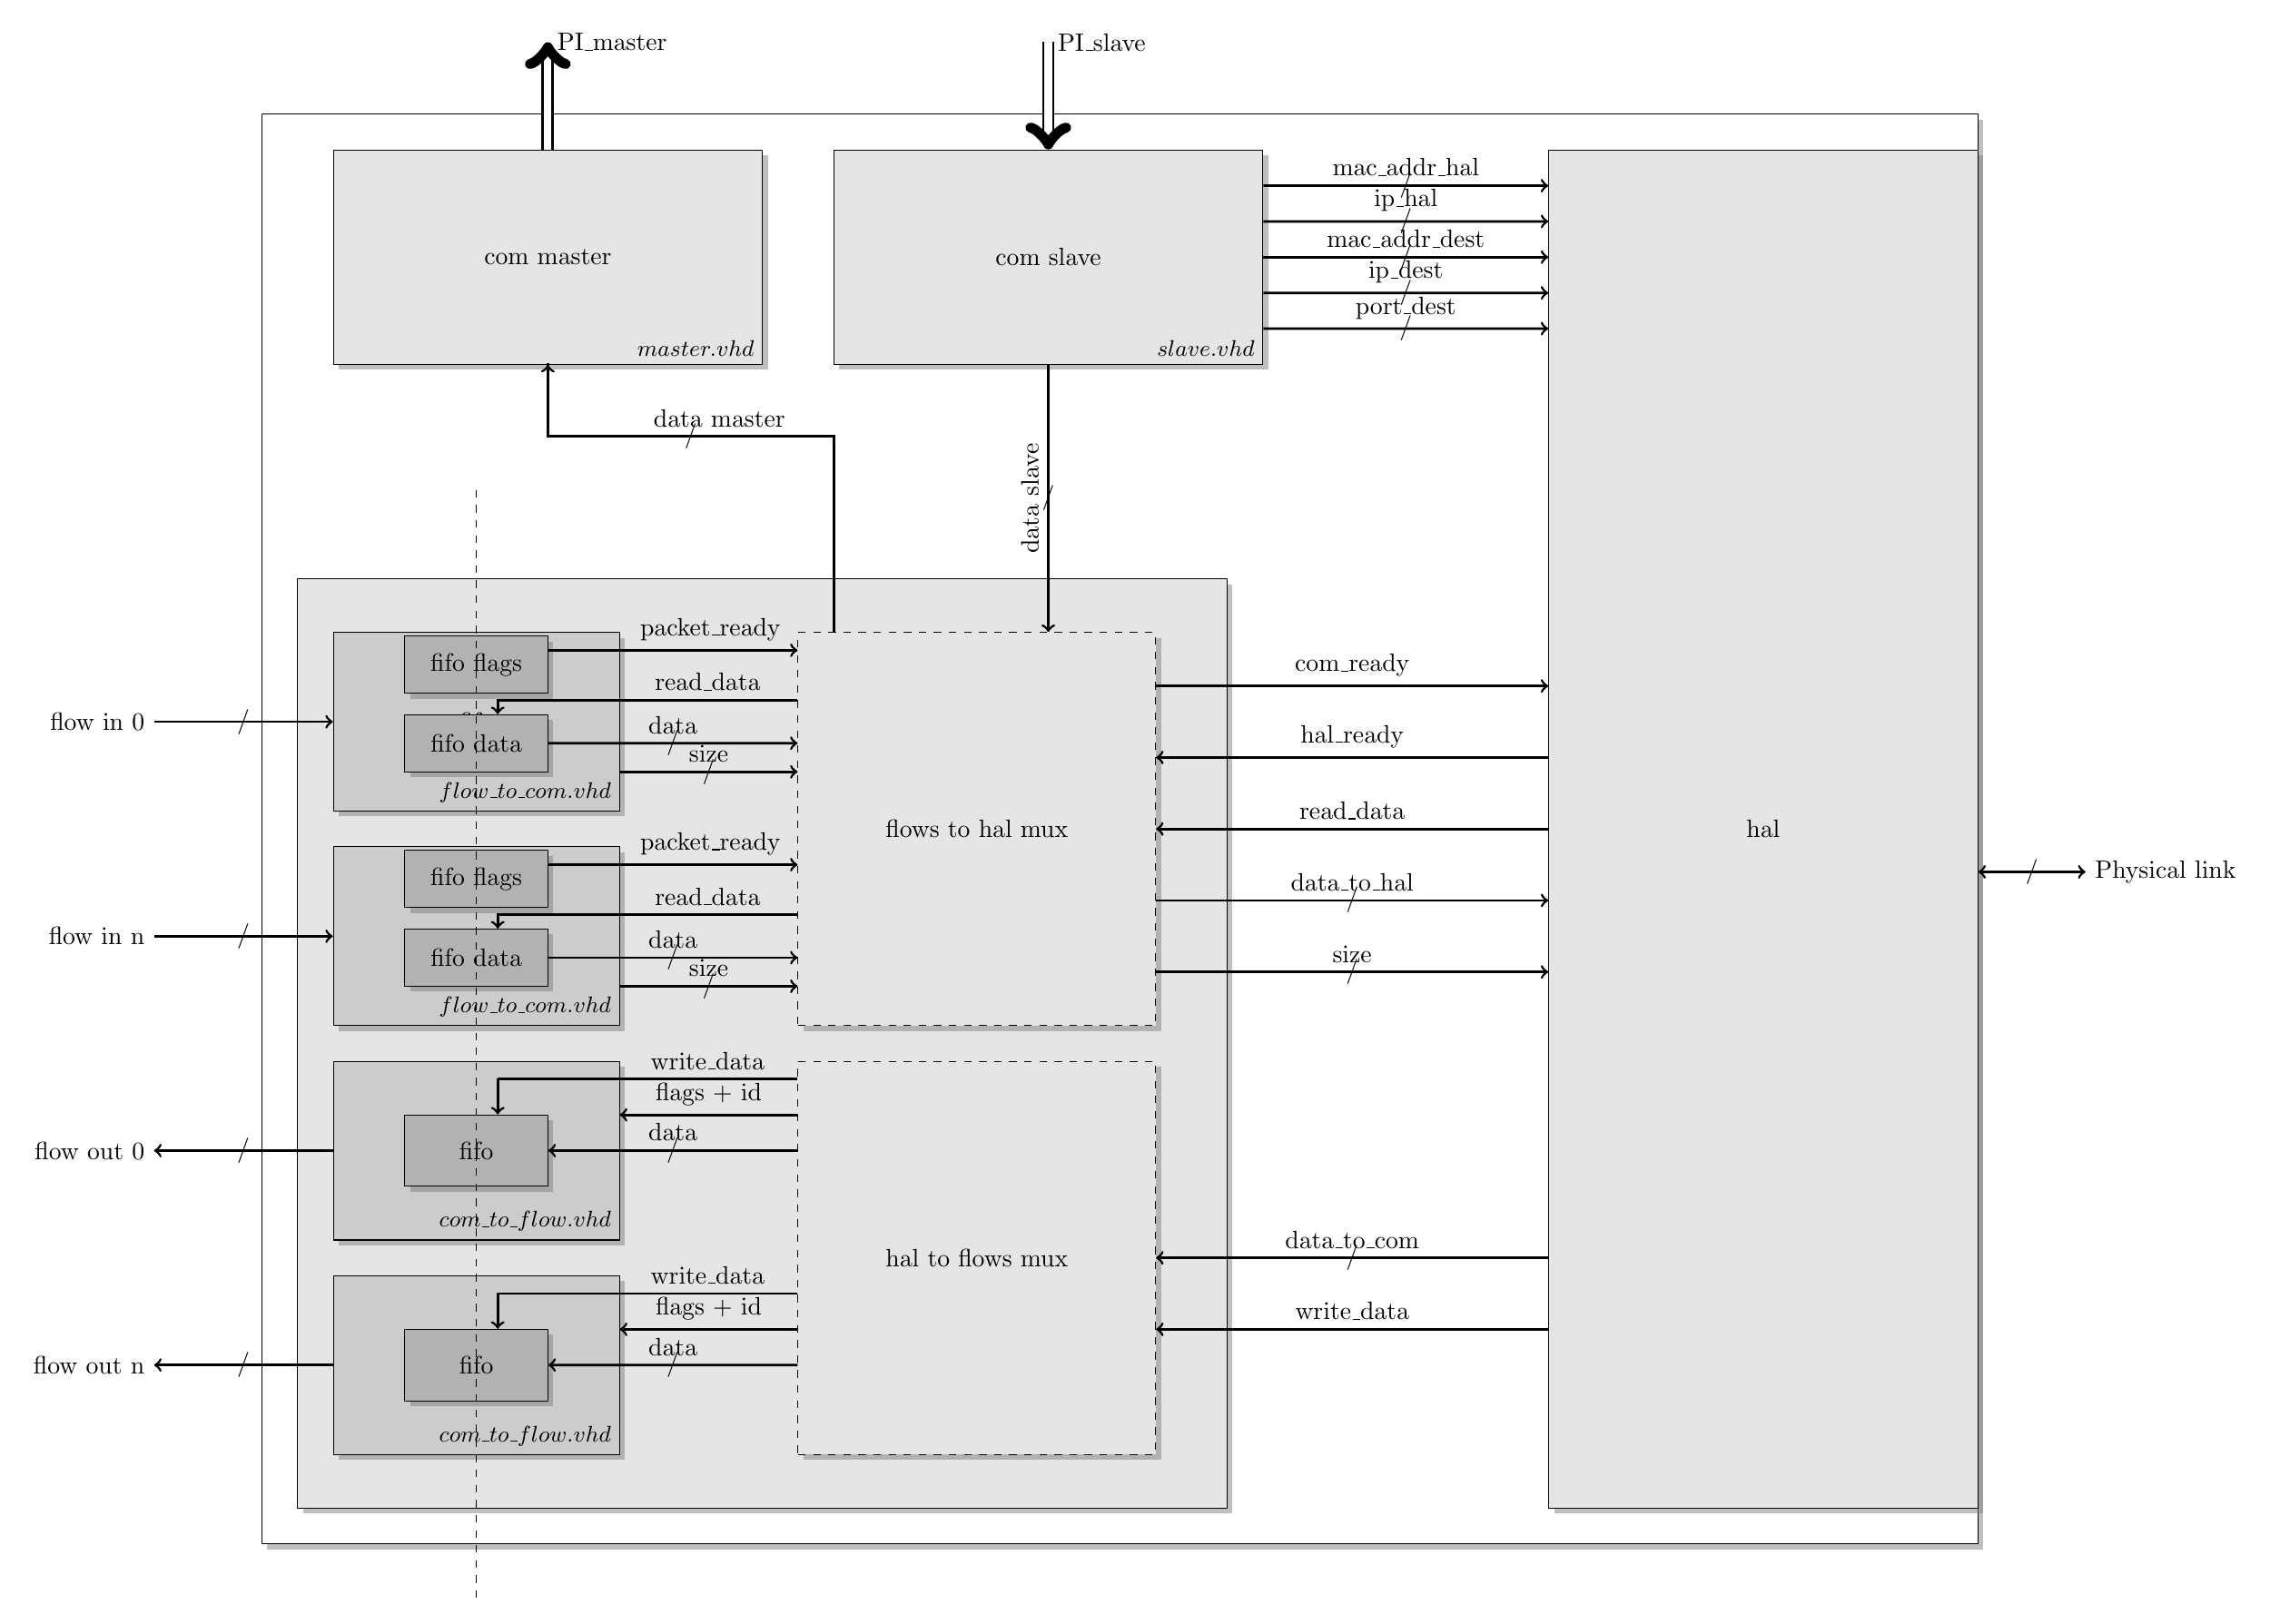
\begin{tikzpicture}



\node[block,minimum height=20cm,minimum width=24cm, fill=white] (bloc) { };

%COM
\node[block,minimum height=13cm,minimum width=13cm, fill=gray!20] (topcom) at([xshift=-5cm,yshift=-3cm]bloc) { };
\draw (topcom.south east) node[above left]{\small } ;

%flow in1
\node[block,minimum height=2.5cm,minimum width=4cm, fill=gray!40] (fifoin) at([xshift=-4cm,yshift=4.5cm]topcom) {fifo};
\node[block,minimum height=0.8cm,minimum width=2cm, fill=gray!60] (fifoin2) at([xshift=0cm,yshift=-0.3cm]fifoin) {fifo data};
\node[block,minimum height=0.8cm,minimum width=2cm, fill=gray!60] (flags1) at([xshift=0cm,yshift=0.8cm]fifoin) {fifo flags};

%flow in2
\node[block,minimum height=2.5cm,minimum width=4cm, fill=gray!40] (fifoin3) at([xshift=-4cm,yshift=1.5cm]topcom) {};
\node[block,minimum height=0.8cm,minimum width=2cm, fill=gray!60] (fifoin4) at([yshift=-0.3cm]fifoin3) {fifo data};
\node[block,minimum height=0.8cm,minimum width=2cm, fill=gray!60] (flags2) at([xshift=0cm,yshift=0.8cm]fifoin3) {fifo flags};
\draw (fifoin.south east) node[above left]{\small $flow\_to\_com.vhd$} ;
\draw (fifoin3.south east) node[above left]{\small $flow\_to\_com.vhd$} ;
\path[connect,<-] (fifoin.west) --  node{/}  ++ (-2.5cm,0) node[left]{flow in 0};
\path[connect,<-] (fifoin3.west) --  node{/}  ++ (-2.5cm,0) node[left]{flow in n};

%flow out1
\node[block,minimum height=2.5cm,minimum width=4cm, fill=gray!40] (fifoout) at([xshift=-4cm,yshift=-1.5cm]topcom) {fifo};
\node[block,minimum height=1cm,minimum width=2cm, fill=gray!60] (fifoout2) at(fifoout) {fifo};
\draw (fifoout.south east) node[above left]{\small $com\_to\_flow.vhd$} ;
\path[connect,->] (fifoout.west) --  node{/}  ++ (-2.5cm,0) node[left]{flow out 0};

%flow out2
\node[block,minimum height=2.5cm,minimum width=4cm, fill=gray!40] (fifoout3) at([xshift=-4cm,yshift=-4.5cm]topcom) {fifo};
\node[block,minimum height=1cm,minimum width=2cm, fill=gray!60] (fifoout4) at(fifoout3) {fifo};
\draw (fifoout3.south east) node[above left]{\small $com\_to\_flow.vhd$} ;
\path[connect,->] (fifoout3.west) --  node{/}  ++ (-2.5cm,0) node[left]{flow out n};

%aiguilleur1
\node[block,minimum height=5.5cm,minimum width=5cm,dashed, fill=gray!20] (com) at([xshift=3cm,yshift=3cm]topcom) {flows to hal mux};
%aiguilleur2
\node[block,minimum height=5.5cm,minimum width=5cm,dashed, fill=gray!20] (com2) at([xshift=3cm,yshift=-3cm]topcom) {hal to flows mux};

%slave master
\node[block,minimum height=3cm,minimum width=6cm, fill=gray!20] (master) at([xshift=-8cm,yshift=8cm]bloc) {com master};
\draw (master.south east) node[above left]{\small $master.vhd$} ;
\node[block,minimum height=3cm,minimum width=6cm, fill=gray!20] (slave) at([xshift=-1cm,yshift=8cm]bloc) {com slave};
\draw (slave.south east) node[above left]{\small $slave.vhd$} ;
\path[connect,<-][double distance = 3pt] (slave.north) --   ++ (0,1.5cm) node[right]{PI\_slave};
\path[connect,->][double distance = 3pt] (master.north) --  ++ (0,1.5cm) node[right]{PI\_master};
\path[connect,->] (slave.south) --  node{/} node[above,rotate=90]{data slave} ([xshift=1cm]com.north);
\path[connect,<-] (master.south) -| ([yshift=-1cm]master.south) -|  node[pos=0.25]{/}  node[above, pos=0.3]{data master} ([xshift=-2cm]com.north);

%hal
\node[block,minimum height=19cm,minimum width=6cm, fill=gray!20] (eth) at([xshift=9cm]bloc) {hal};
\path[connect,<->] ([yshift=-0.6cm]eth.east) --  node{/}  ++ (1.5cm,0) node[right]{Physical link};

%internal signals flowtohal mux
\path[connect,<-] ([yshift=-1cm]eth.west) --  node{/} node[above]{data\_to\_hal} ([yshift=-1cm]com.east) ;
\path[connect,<-] ([yshift=-2cm]eth.west) --  node{/} node[above]{size} ([yshift=-2cm]com.east) ;
\path[connect,->] ([yshift=0cm]eth.west) -- node[above]{read\_data} ([yshift=0cm]com.east) ;
\path[connect,<-] ([yshift=2cm]eth.west) -- node[above]{com\_ready} ([yshift=2cm]com.east) ;
\path[connect,->] ([yshift=1cm]eth.west) -- node[above]{hal\_ready} ([yshift=1cm]com.east) ;

%internal signals haltoflow mux
\path[connect,->] ([yshift=-6cm]eth.west) --  node{/} node[above]{data\_to\_com} ([yshift=0cm]com2.east) ;
\path[connect,->] ([yshift=-7cm]eth.west) -- node[above]{write\_data} ([yshift=-1cm]com2.east) ;
%\path[connect,<-] ([yshift=-4cm]eth.west) -- node[above]{com\_ready} ([yshift=2cm]com2.east) ;
%\path[connect,->] ([yshift=-5cm]eth.west) -- node[above]{hal\_ready} ([yshift=1cm]com2.east) ;

%flowtocom 1
\path[connect,->] (fifoin2.east) -- node[above]{data}  node{/} ([yshift=1.2cm]com.west);
\path[connect,->] ([yshift=0.2cm]flags1.east) -- node[above,pos=0.65]{packet\_ready}  ([yshift=2.5cm]com.west);
\path[connect,->] ([yshift=-0.7cm]fifoin.east) -- node[above]{size} node{/}([yshift=0.8cm]com.west);
\path[connect,->]  ([yshift=1.8cm]com.west)-| ([yshift=0.1cm,xshift=0.3cm]fifoin2.north) node[above,pos=0.15]{read\_data}  -- ([xshift=0.3cm]fifoin2.north)  ;

%flowtocom 2
\path[connect,->] (fifoin4.east) -- node[above]{data}  node{/} ([yshift=-1.8cm]com.west);
\path[connect,->] ([yshift=0.2cm]flags2.east) -- node[above,pos=0.65]{packet\_ready}  ([yshift=-0.5cm]com.west);
\path[connect,->] ([yshift=-0.7cm]fifoin3.east) -- node[above]{size} node{/}([yshift=-2.2cm]com.west);
\path[connect,->]  ([yshift=-1.2cm]com.west)-| ([yshift=0.1cm,xshift=0.3cm]fifoin4.north) node[above,pos=0.15]{read\_data}  -- ([xshift=0.3cm]fifoin4.north)  ;

%comtoflow 1
\path[connect,<-] (fifoout2.east) -- node[above]{data}  node{/} ([yshift=1.5cm]com2.west);
\path[connect,<-] ([yshift=0.5cm]fifoout.east) -- node[above]{flags + id}  ([yshift=2cm]com2.west);
\path[connect,->]  ([yshift=2.5cm]com2.west)-| ([yshift=0.5cm,xshift=0.3cm]fifoout2.north) node[above,pos=0.15]{write\_data}  -- ([xshift=0.3cm]fifoout2.north)  ;

%comtoflow 1
\path[connect,<-] (fifoout4.east) -- node[above]{data}  node{/} ([yshift=-1.5cm]com2.west);
\path[connect,<-] ([yshift=0.5cm]fifoout3.east) -- node[above]{flags + id}  ([yshift=-1cm]com2.west);
\path[connect,->]  ([yshift=-0.5cm]com2.west)-| ([yshift=0.5cm,xshift=0.3cm]fifoout4.north) node[above,pos=0.15]{write\_data}  -- ([xshift=0.3cm]fifoout4.north)  ;

\draw[dashed] ([yshift=-2cm]fifoout3.south) -- ([yshift=2cm]fifoin.north);

%slave to hal
\path[connect,->] ([yshift=1cm]slave.east) -- node{/} node[above]{mac\_addr\_hal}  ([yshift=9cm]eth.west);
\path[connect,->] ([yshift=0.5cm]slave.east) -- node{/} node[above]{ip\_hal}  ([yshift=8.5cm]eth.west);

\path[connect,->] ([yshift=0cm]slave.east) -- node{/} node[above]{mac\_addr\_dest}  ([yshift=8cm]eth.west);
\path[connect,->] ([yshift=-0.5cm]slave.east) -- node{/} node[above]{ip\_dest}  ([yshift=7.5cm]eth.west);
\path[connect,->] ([yshift=-1cm]slave.east) -- node{/} node[above]{port\_dest}  ([yshift=7cm]eth.west);

\end{tikzpicture}


\end{document}